\documentclass[a4paper,12pt,twoside]{report} % głownie z tego sie korzysta, oprocz tego report, book
\usepackage[utf8]{inputenc}
\usepackage{geometry}
\usepackage{polski}
\newgeometry{rmargin=2.5cm,lmargin=2.5cm,tmargin=2.5cm,bmargin=2.5cm}
\usepackage{graphicx}
\usepackage[table,xcdraw]{xcolor}
\usepackage{float}
\usepackage[hyphens, obeyspaces]{url}
\usepackage{amsfonts}
\usepackage{amsmath, amssymb, amsthm}
%\usepackage{hyperref}
\usepackage[final]{pdfpages}
\usepackage{indentfirst}
\usepackage[font={small}]{caption}
\usepackage{caption}
%\captionsetup[sub]{font=normalsize}
\usepackage{subcaption}
\captionsetup{format=hang}
\usepackage[hang,flushmargin]{footmisc}

%\titleformat{\section}{\normalfont\fontsize{12}{12}\bfseries}{\thesection}{1em}{}
%\titleformat{\subsection}{\normalfont\fontsize{12}{12}\bfseries}{\thesubsection}{1em}{}
%\usepackage[T1]{fontenc}
%\usepackage{mathptmx}

\newcommand{\dash}[1]{{\operatorname{\mathit{#1}}}}
%\numberwithin{equation}{section}


\begin{document}
%\maketitle
%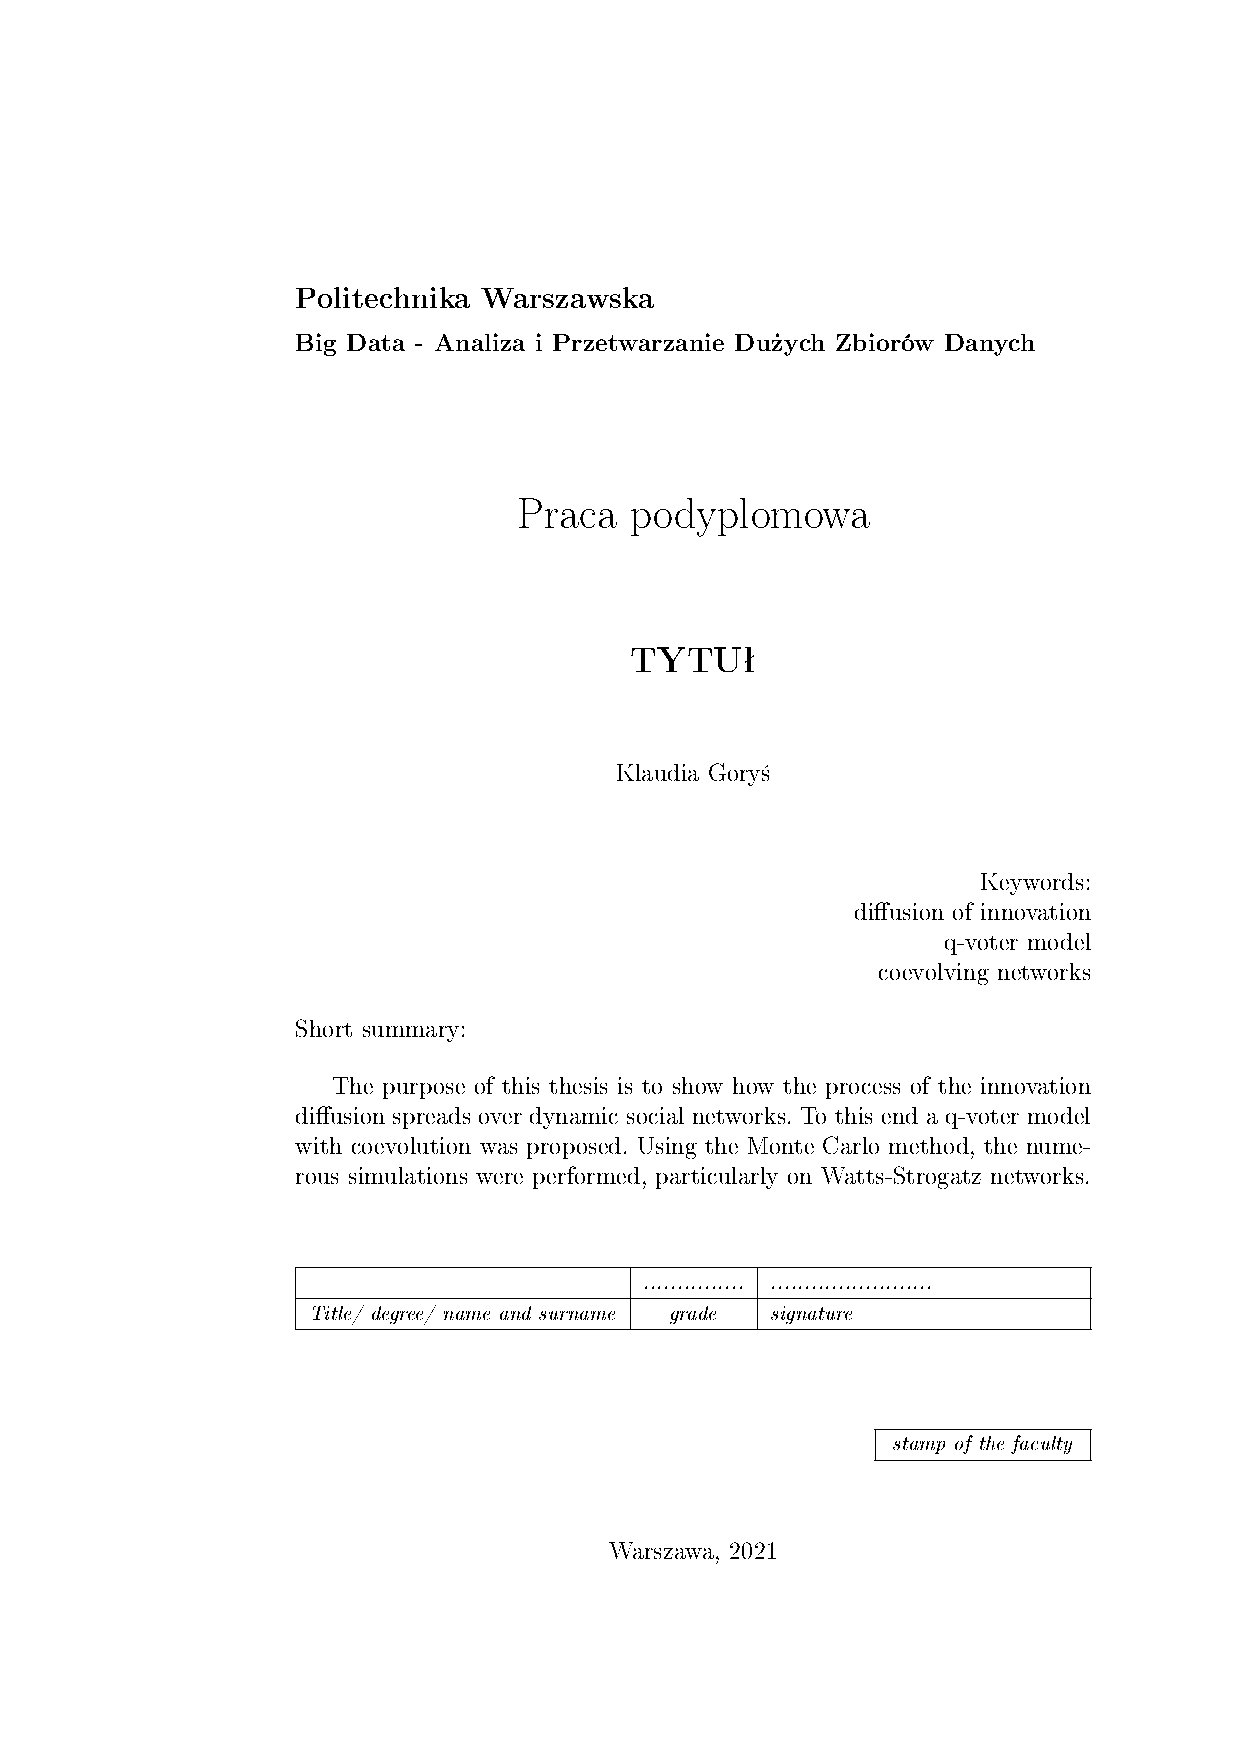
\includepdf{titlepage_eng.pdf}
\tableofcontents

\chapter{Wprowadzenie}
% cel pracy
Celem pracy jest analiza zbioru danych pochodzących ze strony \url{https://archive.org/download/stackexchange}. 

% krotka charakterystyka problematyki
Zbiory danych są skompresowane w folderach dla poszczególnych podstron stackoverflow. Znajdują się w nich pliki xml.
% motywacja
% co chcę pokazać
W pracy chcę odpowiedzieć na pytanie: czy występuje powiązanie pomiędzy zainteresowaniami użytkowników. 


\indent
\section{Amazon Web Services}
Chmura - do czego
Usługi z jakich korzystam: EC2, S3, EMR, ...

\subsection{EC2}


% https://en.wikipedia.org/wiki/File:DiffusionOfInnovation.png
\begin{figure}[H]
\centering
%\includegraphics[width=10cm]{DiffusionOfInnovation.png}
\caption[foot]{Diffusion of innovation curve. \footnotemark[1]}
\label{fig:diffusion_curve}
\end{figure}

\subsection{Storage S3}

\begin{figure}[H]
\centering
%\includegraphics[width=12cm]{diffusion_technology.jpg}
\caption[foot]{The historical adoption of technologies from 1900 until 2005. \footnotemark[2]}
\label{fig:diffusion_technologies}
\end{figure}

In Fig.~\ref{fig:diffusion_technologies} the historical adoption of very 

\footnotetext[1]{Source: \url{https://en.wikipedia.org/wiki/File:DiffusionOfInnovation.png}}
\footnotetext[2]{Source:\url{ https://www.quora.com/Innovation-Diffusion-What-are-the-time-frames-for-adoption}}

\subsection{EMR}

\subsection{PySpark}


\chapter{Projekt}
Dane pobieram ze strony \url{https://archive.org/download/stackexchange}. Następnie chcę je składować na S3. W związku z dużą ilością plików do pobrania, napisałam prosty skrypt w bashu, służący do pobierania danych bezpośrednio ze strony i zrzucaniu ich do folderów na maszynie Ubuntu 20 postawionej na EC2. Następnie pliki są rozpakowywane do folderów. Kolejno pliki: Comments.xml, Posts.xml i Users.xml są przenoszone do bucketów na S3.
Na konsoli CLI puściłam skrypty na screenie w celu szyvszego pobierania danych. Podzieliłam plik z nazwami zbiorów danych na 8 mniejszych. Następnie zdetachedowałam screeny, aby mogły chodzić w tle.

\begin{figure}[H]
\centering
\includegraphics[width=12cm]{bash_script.png}
%\caption[foot]{. \footnotemark[2]}
\label{fig:bash_script}
\end{figure}


\section{EC2} 
EC2 służy do
Wybrałam jeden klaster obliczeniowy na ... Kierowałam się niskimi kosztami maszyny.


\subsubsection{Degree centrality and network's density}

%\begin{equation} \end{equation}


\subsubsection{Average measures}
%\begin{itemize} \item \end{itemize}


\section{Small-world property}


\section{Network models}

\subsection{Random graph}
The very earliest model of a network is an Erdős–Rényi random graph introduced in Ref.~\cite{random_graph}. To build this network, we start with $n$ isolated nodes. Then, for every possible edge, we create the connection with probability $p$. Although very interesting from a theoretical point of view, it is not very popular as a model of 'real-world' networks. In particular, it diverges from the characteristics of social networks.


\subsection{Barabási-Albert model}
Soon after the

\subsubsection{Algorithm}



\chapter{Results}

\section{Fraction of adopted} %over time \ Time coevolution for q-voter model \ Adopted agents over time
\label{sec:qvoter_results}


\begin{figure}[H]
\centering
	\begin{subfigure}[b]{0.49\textwidth}
           \centering
            %\includegraphics[width=\textwidth]{ZZ32_qvoter_coevolution_MC1000_run72legend_w_from00_to04_p005_h008_f01_N100K8.png}
            \caption{Adoption for N=100}   
            \label{fig:adoption_N100_MC1000}
        \end{subfigure}
        \hfill  
        \begin{subfigure}[b]{0.49\textwidth}   
            \centering 
            %\includegraphics[width=\textwidth]{ZZ32_qvoter_coevolution_MC1000_run72legend_w_from00_to04_p005_h008_f01_N500_K8.png}
            \caption{Adoption for N=500}   
            \label{fig:adoption_N500_MC1000}
        \end{subfigure}
        \begin{subfigure}[b]{0.5\textwidth}   
            \centering 
            %\includegraphics[width=\textwidth]{ZZZ_NEW_qvoter_coevolution_MC1000_run80legend_w_from00_to04_p005_h008_f01_N800_K8_beta01.png}
            \caption{Adoption for N=800}   
            \label{fig:adoption_N800_MC1000}
        \end{subfigure}
	\caption{Comparison of adoption process for different network sizes.}   
    \label{fig:adoption_diff_N_MC1000}
\end{figure}


% dlaczego tak sie dzieje? 
From Fig.~\ref{fig:adoption_MC3000} 

In Fig.~\ref{fig:single_trajectories} we present. 

\subsection{Modification of the independence parameter}
Fig.~\ref{fig:averaged_trajectories_for_p_and_f} averaged 


\section{The evolution of networks over time}
\subsection{Characteristic measures} %networks'

The \textit{closeness centrality} is shown in Fig.~\ref{fig:closeness_MC1000_N100}. 


\subsection{The evolution of Watts-Strogatz networks}
Next
     

\subsection{Comparison of network models}
% zbyt wysoka gestosc grafu rowniez utrudnia dyfuzje/
To 

\begin{table}[H]
\centering
\begin{tabular}{|l|c|c|c|c|}
\hline
                       & \textbf{\begin{tabular}[c]{@{}c@{}}average\\ node degree\end{tabular}} & \multicolumn{3}{c|}{\textbf{average clustering coefficient}}                                                                                                                                                                     \\ \hline
\multicolumn{1}{|c|}{} & \textbf{for all w}                                                     & \textbf{\begin{tabular}[c]{@{}c@{}}for all w\\ at t=0 MC\end{tabular}} & \textbf{\begin{tabular}[c]{@{}c@{}}for w=0.05\\ at t=1000 MC\end{tabular}} & \textbf{\begin{tabular}[c]{@{}c@{}}for w=0.15\\ at t=1000 MC\end{tabular}} \\ \hline
\textbf{WS(8, 0.1)}    & 8                                                                      & 0.48                                                                   & 0.15                                                                       & 0.10                                                                       \\ \hline
\textbf{WS(10, 0.1)}   & 10                                                                     & 0.50                                                                   & 0.19                                                                       & 0.12                                                                       \\ \hline
\textbf{BA(4)}   & 7.68                                                                   & 0.17                                                                   & 0.12                                                                       & 0.10                                                                       \\ \hline
\textbf{RN(0.2)}       & 19.78                                                                  & 0.20                                                                   & 0.20                                                                       & 0.20                                                                       \\ \hline
\textbf{RN(0.1)}       & 9.89                                                                   & 0.10                                                                   & 0.11                                                                       & 0.12                                                                       \\ \hline
\textbf{RN(0.08)}      & 7.90                                                                   & 0.08                                                                   & 0.09                                                                       & 0.10                                                                       \\ \hline
\end{tabular}
\caption{Average node degree and average clustering coefficient for different graph models.}
\label{tab:graph_models_measures}
\end{table}


\section{The final concentration of adopted}
 

\subsection{Concentration of adopted as a function of advertising}
First

\subsection{Concentration of adopted as a function of independence}
Results 

\subsection{Critical value of h} 
\label{sec:critical_h}
From Fig.~\ref{fig:Ck_in_h_p005}, we 

\section{Adoption time} % time of adoption
The analysis 

\chapter{Wnioski}
% co zostalo zrobione w poszczegolnych rozdzialach


% najwazniejsze wyniki i wnioski z nich plynace


\nocite{*}
%\bibliography{literature}{}
\bibliographystyle{plain}
{\footnotesize\bibliography{literature}}

\end{document}

